\documentclass[12pt]{article}
\usepackage[utf8]{inputenc}
\usepackage[brazil]{babel}
\usepackage[margin = 1in]{geometry}
\usepackage{graphicx}
\usepackage{subfigure}
\usepackage{minted}
\usepackage{indentfirst}
\usepackage{float}
\usepackage{multirow}


\begin{document}

    
\begin{titlepage}
 \vfill
  \begin{center}
   {\large \textbf{UNIVERSIDADE FEDERAL DO PARANÁ \\ SETOR DE TECNOLOGIA \\ DEPARTAMENTO DE ENGENHARIA ELÉTRICA}} \\[5cm]

  {\large {Marco Antonio Rios  GRR20133243 \\ Wendeurick Silverio GRR20134722} }\\[4cm]


   {\Large \textbf{Projetos de Sistemas Digitais em PLD - TE087} \\ Laboratório 4}\\[6cm]
    \vfill

    \vspace{2cm}

    \large \textbf{Curitiba}

    \large \textbf{\today}

      \end{center}
\end{titlepage}

\clearpage
%\tableofcontents    
%\clearpage

\section{Desafio 1}

O primeiro desafio consiste em um conversor de número codificado em binário para gray. Para converter esse número é possível seguir a seguinte regra:

\begin{figure}[!h]
    \centering
    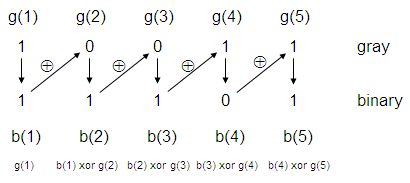
\includegraphics[width=.6\textwidth]{btg.png}
    \caption{Esquema para conversão de binário para código gray}
    \label{fig:btg}
\end{figure}

Deseja-se alcançar um resutado como esse:

\begin{table}[!h]
\centering
\caption{Conversão número binário para gray}
\label{my-label}
\begin{tabular}{|c|c|c|}

\hline
Decimal & Binário & Gray   \\
\hline
0       & 0000    & 0000   \\
1       & 0001    & 0001   \\
2       & 0010    & 0011   \\
3       & 0011    & 0010   \\
4       & 0100    & 0110   \\
5       & 0101    & 0111   \\
6       & 0110    & 0101   \\
7       & 0111    & 0100   \\
8       & 1000    & 1100   \\
9       & 1001    & 1101   \\
10      & 1010    & 1111   \\
11      & 1011    & 1110   \\
12      & 1100    & 1010   \\
13      & 1101    & 1011   \\
14      & 1110    & 1001   \\
15      & 1111    & 1000   \\ \hline 
\end{tabular}
\end{table}

\subsection{Implementação}

Abaixo, o código \emph{VHDL} da implementação.

\inputminted{vhdl}{desafio1.vhd}


\subsection{Mapeamento das portas I/0}
\label{subsec:desafio1_map}

Abaixo, o mapeamento das entradas e saídas para o kit Nexys 2.

\inputminted{vhdl}{pins.ucf}

\subsection{Simulação}

Abaixo, o código \emph{VHDL} do Testbench.

\inputminted{vhdl}{tb_desafio1.vhd}

\begin{figure}[!h]
    \centering
    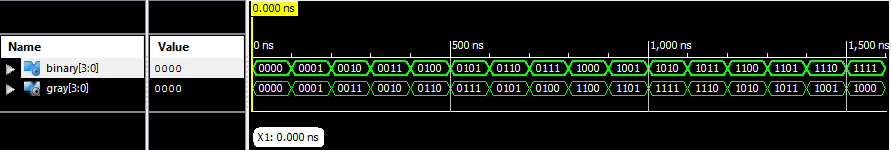
\includegraphics[width=1\textwidth]{tb_1.PNG}
    \caption{Resultado do testbench do desafio 1.}
    \label{fig:desafio1}
\end{figure}

\clearpage

\section{Desafio 2}

O 2º desafio propõe um circuito para a seguinte especificação:

\begin{table}[h]
\centering
\caption{Especificação do Desafio 2.}
\begin{tabular}{|c|l|c|}
\hline
Tipo                      & \multicolumn{1}{c|}{Operação} & Opcode \\ \hline
\multirow{4}{*}{Unsigned} & y = a + b                     & 000    \\ \cline{2-3} 
                          & y = a - b                     & 001    \\ \cline{2-3} 
                          & y = - a + b                   & 010    \\ \cline{2-3} 
                          & y = a + b + cin               & 011    \\ \hline
\multirow{4}{*}{Signed}   & y = a + b                     & 100    \\ \cline{2-3} 
                          & y = a - b                     & 101    \\ \cline{2-3} 
                          & y = - a + b                   & 110    \\ \cline{2-3} 
                          & y = a + b + cin               & 111    \\ \hline
\end{tabular}
\end{table}

onde:
\begin{itemize}
    \item A,B: vetores de entrada
    \item CIN: \emph{carry in}
    \item Y: vetor de saída
    \item COU: \emph{carry out}
    \item OP: selecionador de operação
\end{itemize}

\subsection{Implementação}

Abaixo, o código \emph{VHDL} da implementação.

\inputminted{vhdl}{arithmetic_circuit.vhd}

O compilador emitiu as seguintes mensagens \emph{WARNING}:
\begin{center}
\emph{line 85: Width mismatch. <sSoma> has a width of 9 bits but assigned expression is 8-bit wide.}\\
\emph{line 93: Width mismatch. <uSoma> has a width of 9 bits but assigned expression is 8-bit wide.}
\end{center}

\subsection{Simulação}

Abaixo, o código \emph{VHDL} do Testbench.

\inputminted{vhdl}{arithmetic_circuit_tb.vhd}

Com a implementação anterior, o simulador retornou a seguinte mensagem de erro:
\begin{center}
\emph{ERROR: In process arithmetic\_circuit.vhd:31}\\
\emph{Target Size 9 and source size 8 for array dimension 0 does not match.}
\end{center}

\end{document}
